\chapter{Gitlab On-Premise and Gitlab Cloud}


\section{About Gitlab}

The Gitlab integration supports both on-premise and cloud-hosted Gitlab instances.  Gitlab
considers each "project" as a single code repository.  A project can exist in a "user" or "group"
namespace; projects in a user namespace can be considered an individual repository for \cxoneflow
deployment purposes.  Deploying a webhook to send events to \cxoneflow at the project scope
is possible but would not be ideal for configuring a large number of repositories.

A "group" in Gitlab can contain zero or more projects and zero or more sub-groups. Webhooks
can be configured at a group scope to apply to all projects in the group or sub-groups.  A
licensed version of Gitlab is required to deploy webhook configurations at the group scope.

The on-premise version of Gitlab has "system hooks" that can be utilized to deploy
a single webhook configuration for \cxoneflow.  A system hook will emit events for
all projects in all groups.

Each \cxoneflow service definition for Gitlab will require a PAT that can access repositories
in the scope where webhooks are deployed.  If deploying a system hook, which emits events
for all projects in the Gitlab instance, the PAT will need to belong to an account
that has the appropriate permissions for all projects.  If the webhook is deployed
at the group or project scope, the PAT should have the appropriate permissions
to access the group or project where the webhook configuration is deployed.


\section{\cxoneflowtext\space YAML Configuration for GitLab}

Below is a listing of a minimal Gitlab YAML configuration.  The elements to note in this
configuration:

\begin{itemize}
    \item The \texttt{base-url} is the root URL for the Gitlab instance.  This URL is also used
    when forming display links such as links to code in PR comments.
    \item The \texttt{api-url-suffix} is the path extension appended to \texttt{base-url} for API requests.
    \item The \texttt{repo-match} regular expression matches the service definition with events emitted by any repository
    in the Gitlab instance.
\end{itemize}

\begin{code}{Minimal YAML Configuration Example}{Gitlab Webhooks}{}
  secret-root-path: /run/secrets
  server-base-url: https://cxoneflow.mydomain.com:8443/
  
  gh:
      - service-name: Gitlab
        repo-match: ^http(s)?:(\/){2}gitlab\.corp\.com.*
        feedback:
          pull-request:
            enabled: True
        connection:
          base-url: https://gitlab.corp.com
          api-url-suffix: api/v4
          shared-secret: scm-shared-secret
          api-auth:
            token: ghe-token
        cxone:
          tenant: mytenant
          oauth:
            client-id: my-oauth-id
            client-secret: my-oauth-secret
          iam-endpoint: US
          api-endpoint: US
\end{code}
    

\section{Deploying Webhook Configurations in Gitlab}

The scope where webhooks are deployed for \cxoneflow will determine how to provision a PAT
that has the appropriate permissions to the projects in the deployment scope.  Using service
hooks, for example, requires a PAT from a user that has access to all projects in the Gitlab
instance.

Deploying webhooks at the project or group scope requires a PAT from a user that has access
to the projects in the deployed scope.  This may require multiple \cxoneflow service definitions
with the \texttt{repo-match} regular expression such that events in the scope available to a
PAT are handled properly.

A PAT, regardless of user or scope, requires the following permissions:

\begin{itemize}
  \item api
  \item api\_read
  \item ai features
\end{itemize}

\subsection{Service Hooks}

A Gitlab administrator can configure system-wide service hooks.  The service hooks configuration is located in the
administrative configuration menu, accessible by clicking the "Admin" button as shown in Figure \ref{fig:gl-admin-menu}.

\begin{figure}[ht]
  \centering
  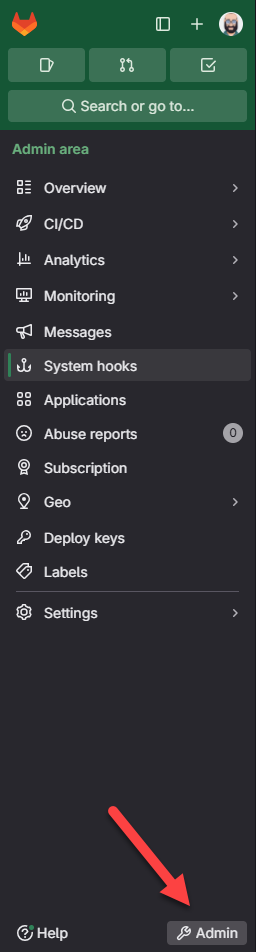
\includegraphics[scale=.5]{graphics/gl-system-hook-admin.png}
  \caption{Gitlab System Hook Administration Menu}
  \label{fig:gl-admin-menu}
\end{figure}


An example service hook definition is shown in Figure \ref{fig:gl-service-hook-def}.  The following are
required configuration elements:

\begin{itemize}
  \item The URL to the \cxoneflow instance ending with the \texttt{gl} route.
  \item The value provided in the \texttt{shared-secret} element under the \texttt{connection} element in the service definition.
  \item The triggers should be \textbf{Push events} and \textbf{Merge request events}.
\end{itemize}

Click the "Add webhook" button to deploy the service hook definition.  Gitlab will immediately start delivering
events to the configured \cxoneflow endpoint.

\begin{figure}[ht]
  \centering
  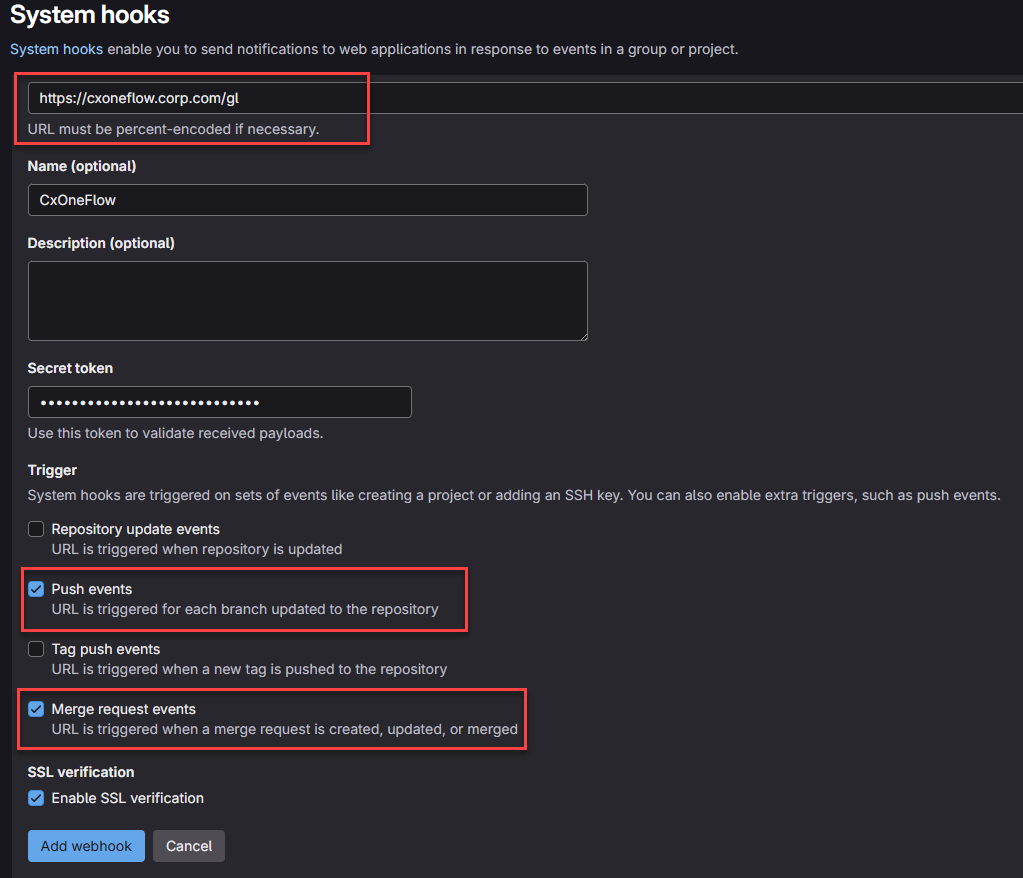
\includegraphics[width=\textwidth]{graphics/gl-service-hooks.png}
  \caption{Gitlab System Hook Definition}
  \label{fig:gl-service-hook-def}
\end{figure}

\subsection{Group or Project Webhooks}

Webhook configurations at the group or project scope operate the same.  The settings for each
are accessed by navigating to the group or project view and selecting \textbf{Settings->Webhooks}.
If attempting to configure webhooks at the group scope in a free Gitlab on-premise instance or
a free Gitlab cloud account, you will be prompted to purchase a license.

The webhook configuration can be initiated by clicking the \textbf{Add new webhook} button. Figure \ref{fig:gl-project-1}
shows the endpoint configuration where the URL for the \cxoneflow instance with the \texttt{gl} is provided
along with the shared secret.  The shared secret value should match the value provided in the
\texttt{shared-secret} element under the \texttt{connection} element in the service definition.

\begin{figure}[ht]
  \centering
  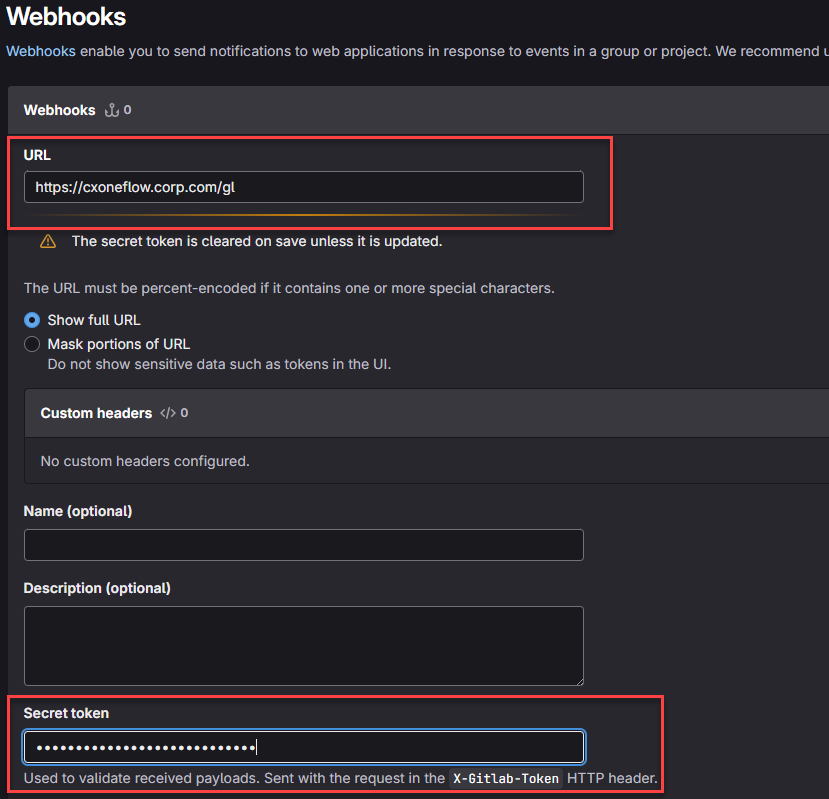
\includegraphics[width=\textwidth]{graphics/gl-project-hook-1.png}
  \caption{Gitlab Group/Project Webhook Endpoint Configuration}
  \label{fig:gl-project-1}
\end{figure}

Figure \ref{fig:gl-project-2} shows the webhook configured to send events for 
\textbf{Push events} and \textbf{Merge request events}.  While it is possible to filter
which branches emit push events, doing so may cause \cxoneflow to not work as expected.

Click the "Add webhook" button to deploy the webhook definition.  Gitlab will immediately start delivering
events to the configured \cxoneflow endpoint.


\begin{figure}[ht]
  \centering
  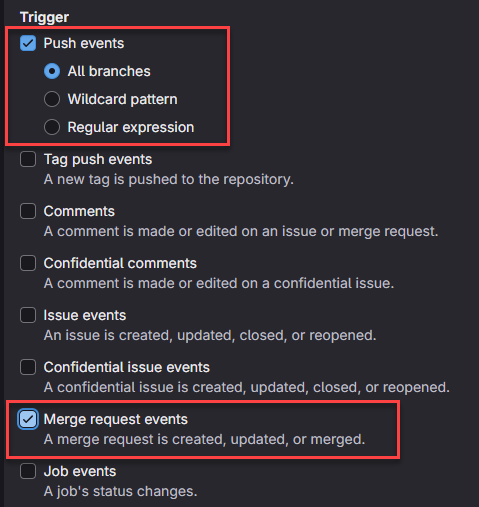
\includegraphics[width=\textwidth]{graphics/gl-project-hook-2.png}
  \caption{Gitlab Group/Project Webhook Event Configuration}
  \label{fig:gl-project-2}
\end{figure}



\section{Protected Branches}

Gitlab allows for a group scope definition of a "default branch" that can be overridden at the
project scope.  The default branch may be considered a protected branch (e.g. it limits who can
commit to the default branch), but Gitlab does not require the default branch to be a protected
branch.  For consistency with \cxoneflow workflow logic with other SCMs, the default branch is
considered a protected branch for all event handling workflows.  This means a push to the 
default branch or a merge request targeting the default branch will initiate a scan regardless
of the configured protection status.

Branch protection rules other than those associated with the default branch can be configured at
the project scope.  The rules allow a named branch to be configured as protected or to supply
a wildcard to protect branches with names that match the wildcard specification.  \cxoneflow will
follow the Gitlab configuration logic for protected branches when handling an event.  Any push
or merge request targeting a protected branch will initiate a scan.
